
    \documentclass{resume}

    \usepackage[left=0.4 in,top=0.4in,right=0.4 in,bottom=0.4in]{geometry}
    \usepackage{tabularx}
    \usepackage{graphicx}
    \usepackage{float}
    \newcommand{\tab}[1]{\hspace{.2667\textwidth}\rlap{#1}} 
    \newcommand{\itab}[1]{\hspace{0em}\rlap{#1}}

    
    \name{Johannes Brandenburger}
    \address{+49 152 1111111 \\ Mengen, Germany}
    \address{\href{mailto:johannes@brandenburger.dev}{johannes@brandenburger.dev} \\ \href{https://linkedin.com/in/johannes-brandenburger}{LinkedIn} \\ \href{https://github.com/johannesbrandenburger}{GitHub} \\ \href{https://resume.example.de}{resume.example.de}}
    \begin{document}

    
        \begin{figure}[H]
        \centering
        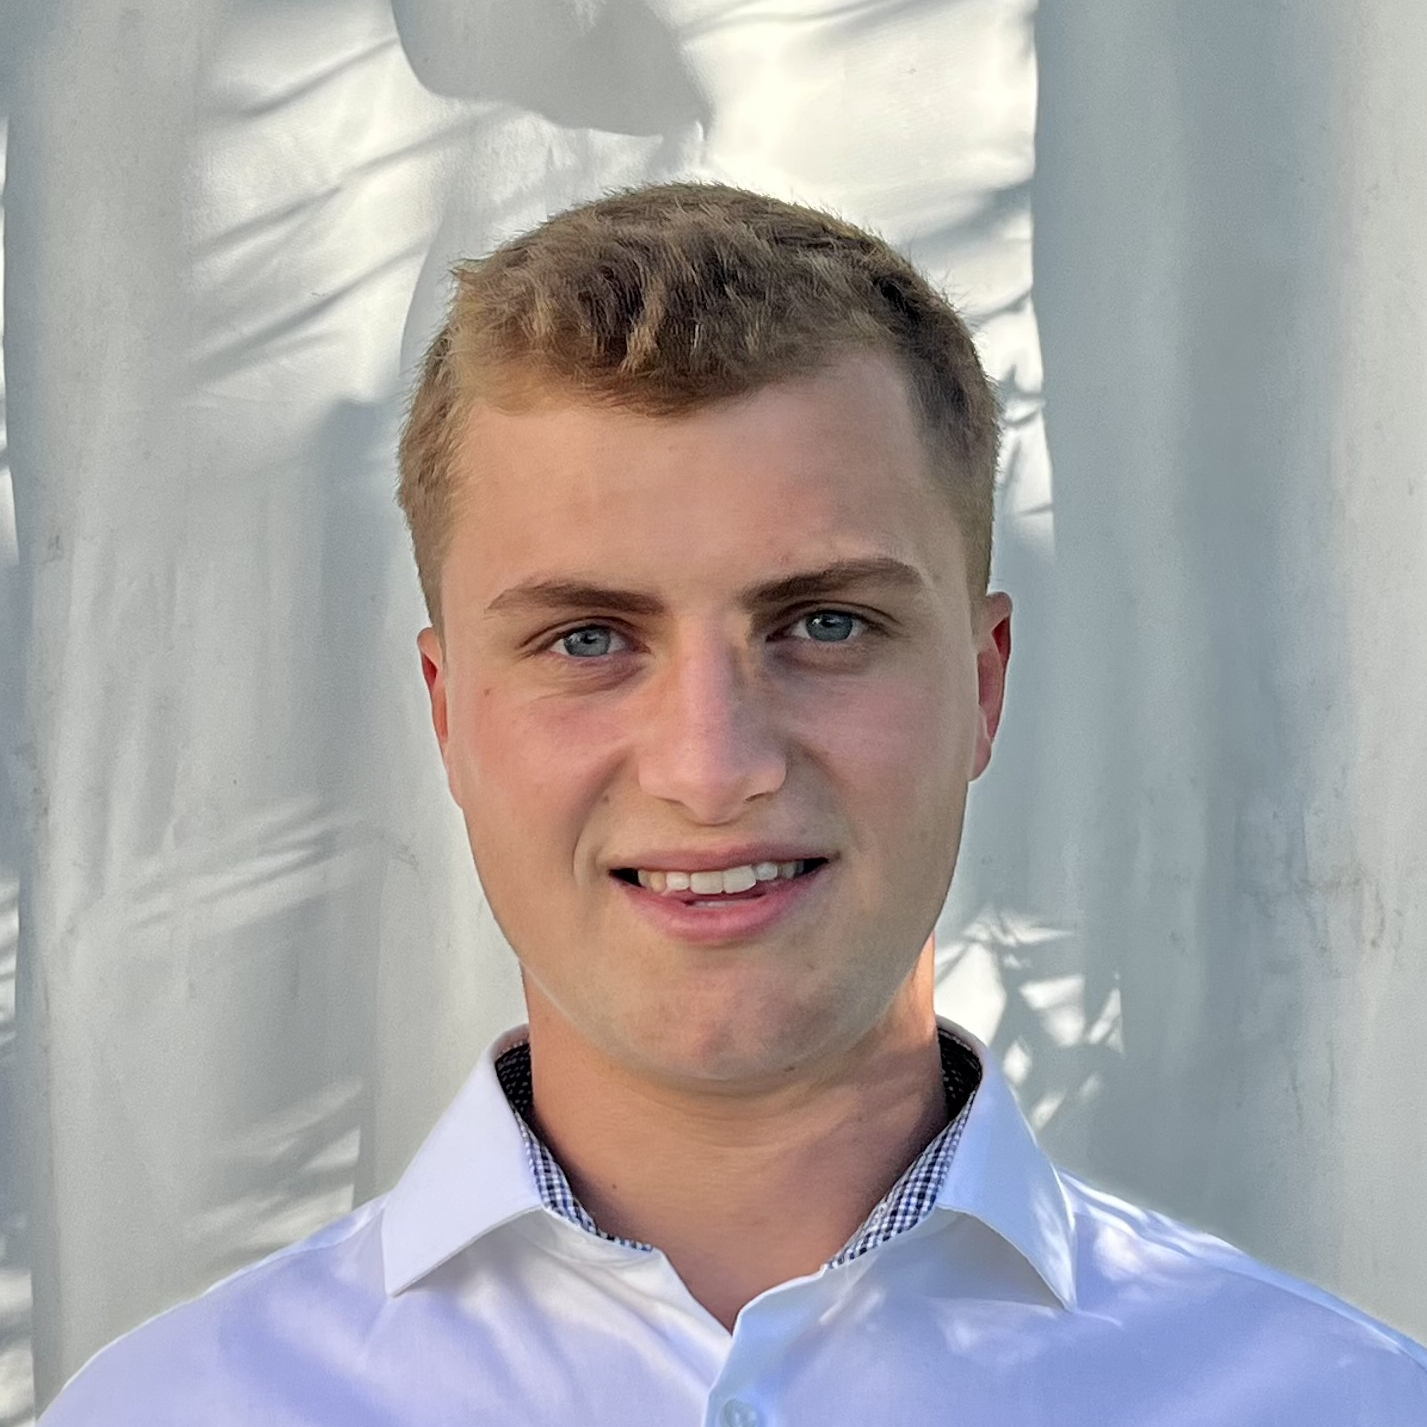
\includegraphics[width=75px]{../web/public/johannes-brandenburger.png}
        \end{figure}
        \vspace{-2em}
        

    \begin{rSection}{OBJECTIVE}

    {I am Johannes, a passionate software developer and engineer. After my dual studies at \href{https://www.example.com/}{Example Company GmbH}, I am currently doing my Master's in Software Engineering in Konstanz, DE. In addition, I work as a freelance developer and consultant for various companies and realize my own side projects in my favorite topics, full-stack development and software architecture. \\\\Currently, I'm developing a resume generator, which is used to generate this resume.}

    \end{rSection}
    
    \begin{rSection}{Education}
    
        {\bf Master of Science in Software Engineering} \hfill {2023 - Expected 2025}\\
        Example University \hfill \textit{Konstanz, Germany}\\
        Current Grade Point Average: \textbf{1.2 (DE) / 3.8 (US-GPA)}

        {\bf Bachelor of Science in Computer Science (Information Technology)} \hfill {2020 - 2023}\\
        Example University \hfill \textit{Mengen, Germany}\\
        Grade Point Average: \textbf{1.3 (DE) / 3.7 (US-GPA)}\\\begin{small}\textit{Thesis: Here should stand the title of the bachelor thesis (1.0 (DE) / 4.0 (US))}\end{small}

    \end{rSection}
    
    \begin{rSection}{SKILLS}
    
    \begin{tabularx}{\linewidth}{@{}>{\bfseries}l@{\hspace{.5em}}X@{}}
        Technical Skills & Java, TypeScript, Python, C++, Docker, Kubernetes, Azure, AWS, TensorFlow, Quarkus, SAP Development \\
        
        Soft Skills & Leadership Qualities ('You take on a very central role in planning and team communication'), Customer Orientation ('Your comprehensible and positive interaction with the CPOs is striking in a positive sense'), Communication Skills ('You communicate with great commitment and authenticity') \\
        
    \end{tabularx}\\
    \end{rSection}
    
    \begin{rSection}{EXPERIENCE}
    
        \textbf{Corporate Student} \hfill Oct 2020 - Sep 2023\\
        \href{https://www.example.com/}{Example Company GmbH} \hfill \textit{München, Germany}
        \begin{itemize}
        \itemsep -3pt {} 
        \item Visited all IT departments of the company
\item Stay abroad to work in a Example subsidiary in Italy for several months
\item Worked on real projects in an international business environment
        \end{itemize}
        
        \textbf{Independent Software Developer and Consultant} \hfill Jan 2018 - Present\\
        Your Own Company \hfill \textit{Konstanz, Germany}
        \begin{itemize}
        \itemsep -3pt {} 
        \item Among others, worked for XXX and YYY.
\item Full-stack development
        \end{itemize}
        
    \end{rSection}
    \newpage
    \begin{rSection}{PROJECTS}
    \vspace{-1.25em}
    
        \item \textbf{Resume All in One}. A web application to generate a web resume as well as a printable PDF version from a JSON file. This resume is generated using this application. Technologies used: Next.js, Aceternity UI and LaTeX. \href{https://github.com/johannesbrandenburger/resume-all-in-one}{(GitHub)} 
        
        \item \textbf{Know Where You Go}. Open-source Google Maps Alternative \href{https://github.com/DHBW-FN-TIT20/know-where-you-go}{(GitHub)} \href{https://know-where-you-go.de}{(Demo)}
        
        \item \textbf{Flight Simulator Online 3D Game}. Developed a 3D game using three.js \href{https://github.com/johannesbrandenburger/flight-simulator-pwa}{(GitHub)} \href{https://flight-simulator.brandenburger.dev}{(Demo)}
        
        \item \textbf{Reveal the World: Cloud Native Travel Map App}. A Web-App with Kubernetes, Terraform, Express, Vue and Leaflet made for running on Azure \href{https://github.com/msi-se/reveal-the-world}{(GitHub)} 
        
        \item \textbf{User Authentication using Voice Recognition}. A student research project concerning the topic of user authentication using voice recognition. \href{https://github.com/DHBW-FN-TIT20/user-authentication-using-voice-recognition}{(GitHub)} 
        
    \end{rSection}
    

    \begin{rSection}{Extra-Curricular Activities}
    \begin{itemize}
    \item Playing drums
\item Alpine skiing
\item Football
    \end{itemize}
    \end{rSection}

    \end{document}
    